% Created 2018-09-18 Tue 19:32
% Intended LaTeX compiler: pdflatex
\documentclass[presentation]{beamer}
\usepackage[utf8]{inputenc}
\usepackage[T1]{fontenc}
\usepackage{graphicx}
\usepackage{grffile}
\usepackage{longtable}
\usepackage{wrapfig}
\usepackage{rotating}
\usepackage[normalem]{ulem}
\usepackage{amsmath}
\usepackage{textcomp}
\usepackage{amssymb}
\usepackage{capt-of}
\usepackage{hyperref}
\usepackage{amsthm, amssymb}
\usepackage{pgf,tikz,pgfplots}
\pgfplotsset{compat=1.15}
\usepackage{mathrsfs}
\usetikzlibrary{arrows}
\usepackage{graphicx}
\usepackage{colortbl}
\usepackage[french, frenchb]{babel}
\pgfplotsset{compat=1.13}
\usepgfplotslibrary{fillbetween}
\newtheorem{property}{Propriété}[section]
\newtheorem{defi}{Défi}[section]
\newtheorem{exe}{Exemple}[section]
\newtheorem{exo}{Exercice}[section]
\newtheorem{sol}{Solution}[section]
\newtheorem{rem}{Remarque}[section]
\newtheorem{demo}[theorem]{Démonstration}
\newcommand{\E}[1]{\ensuremath{\mathbb{#1}}}
\newcommand{\G}[3]{\ensuremath{(\E{#1}^{#2}, #3)}}
\newcommand{\M}[3]{\ensuremath{\left(\mathcal{M}_{#1}(\E{#2}), #3\right)}}
\newcommand{\tc}[2]{\ensuremath{\textcolor{#1}{#2}}}
\usetheme{default}
\usefonttheme{structurebold}
\useinnertheme{rectangles}
\useoutertheme{default}
\author{Laurent Garnier}
\date{}
\title{Cours de 2\up{de} : Fonctions}
\hypersetup{
pdfauthor={Laurent Garnier},
pdftitle={Cours de 2\up{de} : Fonctions},
pdfkeywords={},
pdfsubject={},
pdfcreator={Emacs 25.3.1 (Org mode 9.1.6)},
pdflang={Frenchb},
colorlinks,
citecolor=red,
filecolor=orange,
linkcolor=green,
urlcolor=magenta
}\begin{document}

\maketitle
\begin{frame}{Outline}
\tableofcontents
\end{frame}



\section{\href{http://cache.media.education.gouv.fr/file/30/52/3/programme\_mathematiques\_seconde\_65523.pdf}{Rappels du programme officiel}}
\label{sec:org6e4f36d}
\begin{frame}[label={sec:org2c095bc}]{Rappels du programme}
\begin{description}
\item[{Contenus}] Image, antécédent, courbe représentative
\item[{Capacités attendues}] \begin{itemize}
\item Traduire le lien entre deux quantités par une formule.
\item Identifier la variable et, éventuellement, l'ensemble de
définition.
\item Déterminer l'image d'un nombre.
\item Rechercher des antécédents d'un nombre.
\end{itemize}
\item[{Commentaires}] \begin{itemize}
\item Les fonctions abordées sont généralement des fonctions
numériques d'une variable réelle pour lesquelles l'ensemble
de définition est donné.
\item Quelques exemples de fonctions définies sur un ensemble
fini ou sur \E{N}, voire de fonctions de deux variables (aire
en fonction des dimensions) sont à donner
\end{itemize}
\end{description}
\end{frame}

\section{Traduire le lien entre deux quantités par une formule}
\label{sec:org6a75f35}
\begin{frame}[label={sec:orgc0d524a}]{Modéliser une fonction}
\begin{definition}
\begin{itemize}
\item On définit une fonction f sur un ensemble de nombres D en
associant à chaque nombre x appartenant à D, \alert{un seul} nombre
réel \alert{y}.
\item On dit que f est une fonction de la \alert{variable} x.
\item D est appelé \alert{ensemble de définition} de f (on dit que f \alert{est
définie sur D})
\item On note alors : \[f : x\mapsto y = f(x)\]
\item x est \alert{un antécédent} de y par f
\item y est \alert{l'image} de x par f
\end{itemize}
\end{definition}
\end{frame}

\begin{frame}[label={sec:org1c6960b}]{Avec une courbe}
\begin{exe}
Croissance chinoise (PIB en \%) en fonction du nombre d'années.
\end{exe}

\begin{figure}
\begin{center}
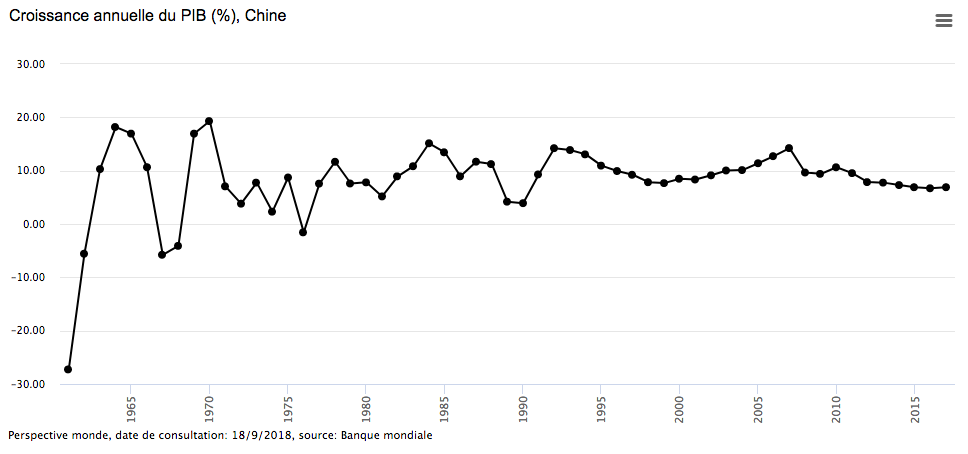
\includegraphics[width=.95\textwidth]{croissance-chinoise.png}
\end{center}
\end{figure}
\end{frame}

\begin{frame}[label={sec:org3321652}]{Avec un tableau de données}
\begin{exe}
Quelle est la distance parcourue pendant le temps de réaction en
fonction de la vitesse ? 

Pour connaître la distance parcourue pendant le temps de réaction,
il suffit de multiplier le chiffre des dizaines par 3. 

\begin{center}
\begin{tabular}{l|r|r|r|r|r}
Vitesse (en km/h) & 50 & 70 & 90 & 110 & 130\\
\hline
Distance (en m) & 15 & 21 & 27 & 33 & 39\\
\end{tabular}
\end{center}
\end{exe}

\begin{defi}
Quelle est la distance parcourue pour une vitesse de 60 km/h ? Pour
80 km/h ? Et pour 100 km/h ?
\end{defi}
\end{frame}

\begin{frame}[label={sec:orgc7d3a34}]{Avec une formule}
\begin{exe}
Au moment où je rédige ce cours le cours du Bitcoin est à 5
446,11€. La formule permettant de déterminer le prix en euros de x
bitcoins est donc : \[f(x) = 5446,11x\]
\end{exe}

\begin{figure}
\begin{center}
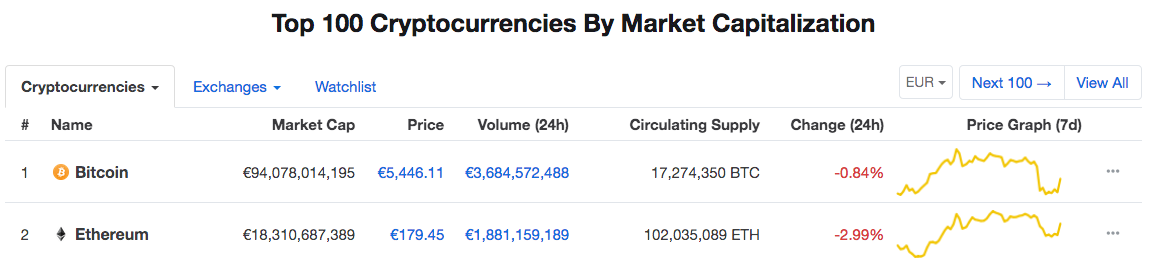
\includegraphics[width=.95\textwidth]{coinmarket.png}
\end{center}
\end{figure}

\begin{defi}
Si 1 BTC = 5 446,11 € quelle fraction de bitcoins obtient-on avec 1
euro ?
\end{defi}
\end{frame}

\section{Courbe représentative d'une fonction}
\label{sec:org4541a73}
\begin{frame}[label={sec:orgdb535d4}]{Une première définition}
\begin{definition}
La fonction f est définie sur D. Dans le plan muni d'un repère, la
courbe représentative \mathcal{C}\(_{\text{f}}\) de la fonction f est l'ensemble
des points M(x;y) tels que y = f(x) quand x prend toutes les
valeurs de D. On dit que \mathcal{C}\(_{\text{f}}\) a pour équation y = f(x).

Cela signifie que :
\begin{itemize}
\item si un point M(x\(_{\text{M}}\) ; y\(_{\text{M}}\)) appartient à la courbe \mathcal{C}\(_{\text{f}}\)
alors y\(_{\text{M}}\) = f(x\(_{\text{M}}\))
\item si y\(_{\text{M}}\) = f(x\(_{\text{M}}\)) alors le point M(x\(_{\text{M}}\) ; y\(_{\text{M}}\)) appartient à la courbe
\mathcal{C}\(_{\text{f}}\)
\end{itemize}
\end{definition}
\end{frame}

\begin{frame}[label={sec:orgb45754f}]{Exemple graphique}
\definecolor{uuuuuu}{rgb}{0.26,0.26,0.26}
\definecolor{qqwuqq}{rgb}{0,0.39,0}
\begin{tikzpicture}[line cap=round,line join=round,>=triangle 45,x=1cm,y=1cm]
\begin{axis}[
x=1cm,y=1cm,
axis lines=middle,
ymajorgrids=true,
xmajorgrids=true,
xmin=-5,
xmax=5,
ymin=-5.25,
ymax=2.75,
xtick={-5,...,5},
ytick={-5,...,2},]
\clip(-5,-5.25) rectangle (5,2.75);
\draw[line width=2pt,color=qqwuqq,smooth,samples=100,domain=-5:5] plot(\x,{0-0.5*(\x)^(3)-(\x)^(2)+3*(\x)+1});
\begin{scriptsize}
\draw[color=qqwuqq] (-3.5,2.25) node {$f$};
\draw [fill=uuuuuu] (0,1) circle (2pt);
\draw[color=uuuuuu] (0.2,.75) node {$A$};
\draw [fill=uuuuuu] (2,-1) circle (2pt);
\draw[color=uuuuuu] (1.75,-0.75) node {$B$};
\end{scriptsize}
\end{axis}
\end{tikzpicture}
\end{frame}
\begin{frame}[label={sec:orge9c67d1}]{Petit exercice}
\begin{defi}
\begin{enumerate}
\item Lire les coordonnées des points A et B sur le graphique
précédent.
\item Combien de fois la courbe passe-t-elle par l'axe des abscisses ?
\item Encadrer chacune des solutions de l'équation f(x) = 0 à l'entier près.
\end{enumerate}
\end{defi}
\end{frame}

\begin{frame}[label={sec:org86fb354}]{Tracer une courbe à partir d'un tableau de données}
On considère le tableau de valeurs suivant :

\begin{center}
\begin{tabular}{l|r|r|r|r|r|r|r}
x & -3 & -2 & -1 & 0 & 1 & 2 & 3\\
\hline
f(x) & 9 & 4 & 1 & 0 & 1 & 4 & 9\\
\end{tabular}
\end{center}


Tracer la courbe représentative associée
\end{frame}
\end{document}